\chapter{Saint Kitts-Nevis}    


\begin{figure}[htbp]
\centering
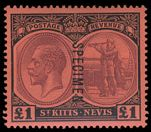
\includegraphics[width=0.35\textwidth]{../st-kitts-nevis/1841.jpg}
\caption{
1841
 SP
\#24-36 (SG24s-36s) 1920-22 KGV \halfd - \pound1 Pictorial set of 13 values 
complete wmk Multiple Crown CA overprinted Specimen. 
LH to HR. F-VF. (Scott \$360, SG \pound350). 
\$      170
} 
\end{figure}  


\begin{figure}[htbp]
\centering
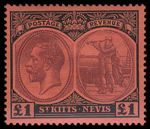
\includegraphics[width=0.35\textwidth]{../st-kitts-nevis/1842.jpg}
\caption{
1842
\#24-36 (SG24-36) 1920-22 KGV \halfd - \pound1 Pictorial set of 13 values 
complete wmk Multiple Crown CA. The 2/6 - \pound1 NH, others OG to HR. F-VF. 
(Scott \$314, SG \pound300). 
\$      140
} 
\end{figure}  

\begin{figure}[htbp]
\centering
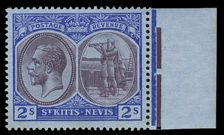
\includegraphics[width=0.45\textwidth]{../st-kitts-nevis/1843.jpg}
\caption{
1843
\#32var (SG32x) 1920-22 KGV 2/ dull purple and blue on blue 
with margin at right, variety watermark sideways reversed. NH. 
F-VF. (SG \pound300). PHOTO
\$      160
} 
\end{figure}  

\begin{figure}[htbp]
\centering
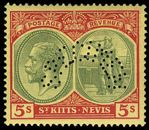
\includegraphics[width=0.45\textwidth]{../st-kitts-nevis/1844.jpg}
\caption{
1844
\#37-51 (SG37s-47bs) 1921-29 KGV \halfd - 5/ complete set of 16 values 
wmk Multiple Crown Script CA perf Specimen. LH to HR. F-VF. (SG \pound400). PHOTO
\$      200
} 
\end{figure}  

\begin{figure}[htbp]
\centering
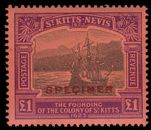
\includegraphics[width=0.45\textwidth]{../st-kitts-nevis/1846.jpg}
\caption{
1846
SP
\#52-64 (SG48s-60s) 1923 \halfd - \pound1 Tercentenary set of 13 values complete
overprinted Specimen. Large part OG to HR. F-VF. (Scott \$775, SG \pound800). PHOTO
\$      425
} 
\end{figure}



\begin{figure}[htbp]
\centering
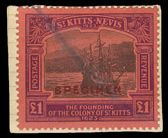
\includegraphics[width=0.45\textwidth]{../st-kitts-nevis/1847.jpg}
\caption{
1847
SP
\#52-64 (SG48s-60s) 1923 \halfd - \pound1 Tercentenary set of 13 values 
complete overprinted Specimen affixed to piece, each with blue diagonal 
line. Inscription on reverse of \pound1 states Specimen set from record 
book of ( ) administration. F-VF. (Scott \$775, SG \pound800). PHOTO
\$      450
} 
\end{figure}

\begin{figure}[htbp]
\centering
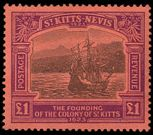
\includegraphics[width=0.45\textwidth]{../st-kitts-nevis/1848.jpg}
\caption{
1848

\#52-64 (SG48-60) 1923 \halfd - \pound1 Tercentenary set of 13 values complete, 
the 10/ with margin at right. Most LH. Fresh. F-VF. (Scott \$1,453, SG \pound1,200). 
PHOTO INSIDE BACK COVER
\$      700
} 
\end{figure}

\begin{figure}[htbp]
\centering
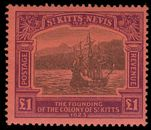
\includegraphics[width=0.45\textwidth]{../st-kitts-nevis/1849.jpg}
\caption{
1849
\#64 (SG60) 1923 \pound1 black and purple on red 
Tercentenary high value. OG. Fine+. (Scott \$875, SG \pound800). PHOTO
} 
\end{figure}

\begin{figure}[htbp]
\centering
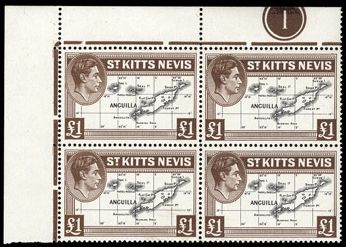
\includegraphics[width=0.65\textwidth]{../st-kitts-nevis/1850.jpg}
\caption{
1850
\#79-90 (SG68a-77c) 1938-50 KGVI \halfd - \pound1 set of 12 values complete in blocks of 4, 
most with margin, the 10/ and \pound1 with UL corner margin control number. 
The 1/, 2/6 and 5/ are chalky papers. NH except one 10/ and one \pound1.
F-VF. (SG \pound476).
\$  250
} 
\end{figure}    


                    